\documentclass{report}

%-------------[oneside,12pt]-----------------Zone 1-------------------------
\usepackage{ebgaramond}
\usepackage{graphicx}
\usepackage{epigraph}
\usepackage[utf8]{inputenc} % un package permet d'utiliser tous les caractères de votre clavier.
\usepackage[T1]{fontenc} % un second package permettant d'utiliser tous les caractères de votre clavier.
%\usepackage[francais]{babel} % un troisième package pour dire à <em>Latex</em> que vous écrivez en français.
\usepackage{fancyhdr}



%------------------------------Fin Zone 1---------------------------

\begin{document}

%------------------------------Zone 2: début des page non numérotées-------------------------

\sloppy
\begin{titlepage}
\begin{center}
{\bf People's Democratic Republic of Algeria
\\Ministry of Higher Education and
Scientific Research} \vspace{0.25cm}\\
{\bf {\large University of Batna 2}}\\
{\bf Faculty of Mathematics and Computer Science} \\ {\bf Department of Computer Science}\\
\vspace{0.2cm}
\Huge{\emph{{{\it {End Of Study Thesis }}}}}\\
\vspace{0.1cm}
\normalsize
\begin{center}
In order to obtain the computer license\\

\end{center}
\normalsize\textbf{Option }:\\
\normalsize
\begin{center}
Information Systems Engineering and Software
\end{center}
\vspace{0.09cm}
\Huge\textbf{Theme}\\
\noindent\rule{\textwidth}{0.9mm}
\Large{{\textbf{COVID-19\\ Data Visualisation}}}
\noindent\rule{\textwidth}{0.9mm}
\end{center}
\begin{center}
\normalsize %\hspace{-2cm}
\begin{tabular}{llll}
\vspace{0.09cm}
\hspace{5.1cm}
\hspace{4.9cm} 
\\
\hspace{5.1cm}
\\\\
%\vspace{1.5cm}
\textbf{Présenté par: \hspace{0cm}}~~~~~~~~~~~~\\\\
%\vspace{0.1cm}
\textbf{\textbf{$M^{r}$ Houssam HAMOUDA }}\\
\textbf{\textbf{$M^{r}$ Aziz HAGAIN }}\\
\textbf{\textbf{$M^{r}$ Chaker DIAB }}\\
\textbf{\textbf{$M^{r}$ Mourad MAAZOUZA }}\\
\textbf{\textbf{$M^{r}$ Abdeladhim ZAOUI }}

\end{tabular}
\end{center}
\vspace{0.12cm}
\begin{center}
academic year 2020/2021
\end{center}
\end{titlepage}
\chapter*{Thanks}
\thispagestyle{empty}

Throughout the drafting of this brief, I received a great deal of support and assistance.

I would like to begin by thanking our coach, Dr. Redha Abdessmad, whose expertise has been invaluable in formulating the research questions and methodology. Your insightful comments have prompted me to refine my thinking and elevate my work to a higher level.

I want to thank my colleagues for their wonderful collaboration. I would especially like to acknowledge the team of the Computer Science Department, the Dean, the Head of Department and all the teachers, I would like to thank you for your support to the patients and for all the opportunities that have been given to me to continue my research.\\
I would also like to thank my employer and co-workers
\chapter*{Dedication}
\setlength\epigraphwidth{.6\textwidth}
\setlength\epigraphrule{0pt}

\thispagestyle{empty}
\vspace*{\fill}
\epigraph{\itshape «Dedicated to all Frontline Workers.»}



\chapter*{Summary}
\thispagestyle{empty}


\section*{What is web development?}
Web development generally refers to tasks associated with the development of websites to
be hosted via an intranet or the Internet. The web development process includes, but is not
limited to, website design, web content development, client or server-side scripting and
network security configuration.\\

Web development is the coding or programming that makes a website work, according to the
owner’s requirements. It focuses on the non-conceptual aspect of website creation, which
includes coding and writing markup.
Web development ranges from the creation of plain text pages to complex web applications,
social networking applications and electronic business applications.
\section*{Data Visualisation}
Visualization techniques have been front-and-center in the efforts to communicate the science around COVID-19 to the very broad audience of policy makers, scientists, healthcare providers, and the general public.\\

In this article, I summarize and illustrate how visualization can help understand different aspects of the pandemic.


%------------------------------Fin Zone 2: fin des page non numérotées---------------------------

%------------------------------Zone 3:début entêtes et prieds de page-----------------------------------------

\pagestyle{fancy}.
\renewcommand{\footrulewidth}{1pt}
\fancyhead[L]{\thesection}


\fancyfoot[C]{\textbf{page \thepage}}
\fancyfoot[R]{COVID-19 Data Visualisation}

%------------------------------Fin Zone 3: fin des entêtes et prieds de page-------------------------------------------

%-----------------Zone 4: début de la numérotation avec les chiffres romains-----------------

\tableofcontents

\pagenumbering{roman}%numérotation avec les chiffres romains
\setcounter{page}{1} %début de la numérotation est 1.

\listoftables
\addcontentsline{toc}{chapter}{Liste des tableaux}
\listoffigures
\addcontentsline{toc}{chapter}{Table des figures}

\chapter*{Liste des abréviations}
\addcontentsline{toc}{chapter}{Liste des abréviations} % rajoute la liste des abréviations.

%-----------------Fin Zone 4: fin de la numérotation avec les chiffres romains-------------------

%-----------------Zone 5: début de la numérotation avec les chiffres arabs-------------------

%
\section*{What is web development?}
Web development generally refers to tasks associated with the development of websites to
be hosted via an intranet or the Internet. The web development process includes, but is not
limited to, website design, web content development, client or server-side scripting and
network security configuration.\\

Web development is the coding or programming that makes a website work, according to the
owner’s requirements. It focuses on the non-conceptual aspect of website creation, which
includes coding and writing markup.
Web development ranges from the creation of plain text pages to complex web applications,
social networking applications and electronic business applications.
\section*{Data Visualisation}
Visualization techniques have been front-and-center in the efforts to communicate the science around COVID-19 to the very broad audience of policy makers, scientists, healthcare providers, and the general public.\\

In this article, I summarize and illustrate how visualization can help understand different aspects of the pandemic.


\pagenumbering{arabic}% numérotation avec les chiffres arabe
\setcounter{page}{1} % début de la numérotation est 1.


\chapter{Data Visualisation}
\section{Definition}.
Data visualization is the graphical representation of information and data. By using visual elements like charts, graphs, and maps, data visualization tools provide an accessible way to see and understand trends, outliers, and patterns in data.\\

In the world of Big Data, data visualization tools and technologies are essential to analyze massive amounts of information and make data-driven decisions
THE DEADLY IMPACT of COVID-19 is driving a massive amount of research that aims at understanding the various characteristics of the pandemic. While there is no vaccine, considerable effort has been devoted to understanding the spread of the disease in different places in the world. The speed with which the disease has spread throughout the world demands agile solutions to understand and estimate the disease progression.\\

Interactive dashboards with several charts surfaced in different formats to offer concise ways to express the pandemic’s growth. Figure 1.1 illustrates some examples. The dashboard developed by Johns Hopkins University (JHU)1 was the first to track and display information on cases and death totals for different countries and states in the United States.\\

Along with lists of total counts and histograms, a bubble map composed of circles of different radii allows a visual inspection of how serious the pandemic is around the world.\\

Interesting plots were created on news outlets such as the New York Times (NYT)2,3 and the Washington Post.3 For example, NYT used Choropleth maps, a representation where geographical regions (countries or states) are mapped to colors associated with a measurement for that region (e.g., number of cases).\\

This representation is useful to communicate trends, such as the average daily counts for the past week. Similarly, they display the time series evolution for each region using line heatmaps, where daily values are mapped to colors and displayed in a row.\\

Our work (described in more detail in the following) used both Choropleth maps and line heatmaps in the development of dashboard specially designed for Brazil. Using a focus-pluscontext interface with coordinated views, the user can inspect the context using two Choropleth maps (one for the states and a second for a state selected), as well as details using two matrix heatmaps (collection of stacked line heatmaps) for states and cities. The tool displays daily or cumulative data, absolute or relative to population, and supports filtering by a time interval.\\

A vast collection of community-developed dashboards and interactive tools about COVID19 are available. Good starting places to look are the data hub hosted by Tableau and the top 100 R-resources organized by Soetewey.4 In-depth analysis is available at sites, such as Our World in Data, 5 Bing, 6 and the COVID Tracking Project, 7 among others. After developing the Brazilian dashboard, we devoted our efforts to create a set of tools to compare the spread of COVID-19 data in different regions of the world.8 We collected data from more than 6 000 locations in the world, and our interface has different charts that support visualizing multiple locations in a single chart.\\

Since the pandemic is at different stages in the world, we allow the user to align the time-series of data by a certain data the series passes a given threshold (e.g., after 100 cases). This representation is useful to observe when different locations passed through specific checkpoints (top of Figure 2).\\

While our initial charts support the comparison of different regions, the tool required the user to drive the process of choosing the regions to compare.\\

From the beginning, we felt the need to have an automatic tool that could, given a region of interest, return the closest regions given a similarity function. Looking at the disease’s spread in distinct places, but with similar growth patterns, can be useful to predict behaviors.\\

Thus, we developed a search engine to support queries using different similarity functions. For example, at the bottom of Figure 2, we show the results of searching for regions similar to Italy concerning the number of deaths.\\

The results are listed in a ranking, with pairwise comparisons that detail attributes of the different locations and evolution charts, aligned by the day of the first death. We observe the similarities in the evolution in the number of deaths and cases for Italy, France, Spain, and the United Kingdom.\\

While using the tool, we also saw similarities among cities from Brazil and the United States, both countries with large COVID-19 numbers.\\

The examples so far give a glimpse of how data visualization can help in the understanding of COVID-19. Figure 3 illustrates other applications where data visualization can help. The first example shows how multidimensional projections and network visualizations can help the literature exploration of papers that describe novel coronavirus research.\\

As new research about COVID-19 is published, there is a great need to review up-to-date literature and treatments conveniently.\\

Contact tracing is another application that relies on graph visualization to trace the network of people who may have been in contact with a COVID-19 patient, an activity essential to control the dissemination of the disease and essential for directing social distancing regulations. Graph visualization is also important in for social media spread and fact checking. \\

With many people at home, social networks are playing a significant role in people’s lives these days. Unfortunately,.\\

the dissemination of fake news and automated posting from robots is also rising. Fact-checking over the propagation network can help identify misleading information and patterns of dissemination.\\

The fourth and final example highlights the importance of data visualization in the analysis of scientific simulations.\\

It shows the visualization of simulating the transport and spread of novel coronavirus in closed spaces,9 which shows how an infected person can disseminate the virus indoors.\\

Many other examples include data visualization in the analysis of COVID-19 data, and many more is surfacing every day. We hope this summary highlights interesting examples, give pointers to other references, and motivate people to pursue other applications. 
\section{The advantages and benefits of good data \\ visualization}
Our eyes are drawn to colors and patterns. We can quickly identify red from blue, square from circle. Our culture is visual, including everything from art and advertisements to TV and movies.\\

Data visualization\cite{dataviz} is another form of visual art that grabs our interest and keeps our eyes on the message. When we see a chart, we quickly see trends and outliers. If we can see something, we internalize it quickly. It’s storytelling with a purpose. If you’ve ever stared at a massive spreadsheet of data and couldn’t see a trend, you know how much more effective a visualization can be.\\

As the “age of Big Data” kicks into high-gear, visualization is an increasingly key tool to make sense of the trillions of rows of data generated every day. Data visualization helps to tell stories by curating data into a form easier to understand, highlighting the trends and outliers. A good visualization tells a story, removing the noise from data and highlighting the useful information.\\

However, it’s not simply as easy as just dressing up a graph to make it look better or slapping on the “info” part of an infographic. Effective data visualization is a delicate balancing act between form and function. The plainest graph could be too boring to catch any notice or it make tell a powerful point; the most stunning visualization could utterly fail at conveying the right message or it could speak volumes. The data and the visuals need to work together, and there’s an art to combining great analysis with great storytelling.


\section{Why data visualization is important for any career}
It’s hard to think of a professional industry that doesn’t benefit from making data more understandable. Every STEM field benefits from understanding data—and so do fields in government, finance, marketing, history, consumer goods, service industries, education, sports, and so on.
While we’ll always wax poetically about data visualization (you’re on the Tableau website, after all) there are practical, real-life applications that are undeniable. And, since visualization is so prolific, it’s also one of the most useful professional skills to develop. The better you can convey your points visually, whether in a dashboard or a slide deck, the better you can leverage that information.
The concept of the citizen data scientist is on the rise. Skill sets are changing to accommodate a data-driven world. It is increasingly valuable for professionals to be able to use data to make decisions and use visuals to tell stories of when data informs the who, what, when, where, and how. While traditional education typically draws a distinct line between creative storytelling and technical analysis, the modern professional world also values those who can cross between the two: data visualization sits right in the middle of analysis and visual storytelling.
\section{The different types of visualizations}
When you think of data visualization, your first thought probably immediately goes to simple bar graphs or pie charts. While these may be an integral part of visualizing data and a common baseline for many data graphics, the right visualization must be paired with the right set of information. Simple graphs are only the tip of the iceberg. There’s a whole selection of visualization methods to present data in effective and interesting ways.\\

\textbf{Common general types of data visualization:}
\begin{itemize}
\item Charts;
\item Tables;
\item Graph.
\item Maps.
\item Infografics.
\item Dashboards.
\end{itemize}

\begin{figure}[htbp]
\centerline{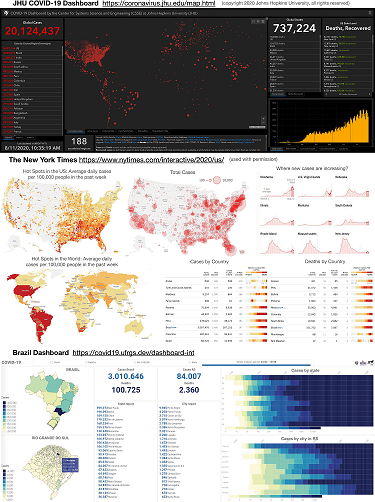
\includegraphics{Chapitre1/dashboard.png}}
\caption{Examples of data visualization in action.}
\label{fig}
\end{figure}

\chapter{JavaScript Charting For Dataviz}
\section{Introduction}
Data must Be analysed and visualized, to turn data into insights , So, here's the question: \textbf{how to pick the right tool?}\\

In this chapter we're going to go through JavaScript frameworks and libraries that you can use to visualize our data. And I'd like to do a bit more than just list a few frameworks — I'm going to divide the list by the type of data or data visualization because "one size" doesn't fit all. There are different kinds of data, and each needs a specific visualization strategy.
\begin{enumerate}
    \item General-purpose charting libraries
    \item Low-level and complex charting libraries
    \item tables and data grids
    \item Timeline charts and time-based tools
    \item Geospatial and mapping tools
    \item Word clouds
    \item 3D visualization tools
\end{enumerate}
 
\section{General-purpose charting libraries}
\subsection{ChartJs}
The most popular open-source library \cite{rajvsp2019approach}for building responsive bar, pie, and line charts. I'd say this is the go-to library for most of the projects, as it fits most of the use cases.
\subsection{Recharts}
A composable charting library built on React components \\

As per description, "It was built on top of SVG elements with a lightweight dependency on D3 submodules." It's a good choice for React-based projects, because you can use it natively as a component.
\subsection{Highcharts}
Highcharts is a JavaScript charting library based on SVG, with fallbacks to VML and canvas for old browsers.\\

Highcharts is good for large companies whose products rely heavily on data visualization. You can see the code on GitHub, try and use it for non-commercial purposes. And then you can purchase Highcharts license just for Hightcharts or Highcharts plugin for Stocks, Maps, or Gantt if you'd like to use it for commercial purposes. We'll cover those later in this post as well.
\subsection{Chartist.js}
Chartist.js is the product of a community that was disappointed about the abilities provided by other charting libraries.\\

This library is not as actively maintained as others, however, it still worths a mention because of its size with no dependencies. Less than a megabyte.\\

Just like others, it uses SVGs, it's flexible and it has clear separation of concerns, i. e., CSS is in CSS and JS is in JS, which may not fit all projects, considering that a lot of projects are using CSS-in-JS approach, yet it still deserves our attention.
\subsection{React-vis}
A collection of React components to render common data visualization charts, such as line/area/bar charts, heat maps, scatterplots, contour plots, hexagon heatmaps, pie and donut charts, sunbursts, radar charts, parallel coordinates, and tree maps.\\

This library is React-friendly, high-level and customisable, expressive and industry-strong, because it is backed by Uber, so chances are you'll get your answers in case you bump into an issue.
\newpage
\subsection{amCharts}
A go-to library for data visualization. When you don't have time to learn new technologies.\\

This is not as popular as the rest, however, it's actively maintained and claims to be easy to use. It could be a good choice if you'd like to combine it with other data viz library for geo and timeline data. I'll cover those in Geo and Timeline sections.\\

Many other library may exist such as D3.js and Leaflet ,but in our project , we choose amCharts Library for our dataViz because it contain interactive timelines easy to manipulate. 

\section{Using amCharts}
amCharts have a wide selection of charts type, including geographical maps, and since it was designed to work with modern web dev toolkits like React, Angular, Vue, Ember, it will just fall into place, right out of the box.\\
\subsection{X/Y}
Line, Smoothed line, Area, Column / 3D column, Bar / 3D bar, Curved column, Cylinder, Cone, Scatter, Bubble, Candlestick, OHLC, Step (incl. w/ no-riser), Floating, Waterfall, Error, Stacked (regular, 100\% or 3D), Heatmap, GANTT, and any combination of these.
\subsection{Sliced}
Pie, 3D pie, Donut, Nested donut, Sunburst, Funnel, Pyramid, Pictorial.
\subsection{Geo Maps}
Map chart, Geo heat map, Map combined with charts. (Maps is an add-on and requires separate license)
\subsection{Other}
Sankey diagram, Treemap, Chord diagram, Radar, Polar.
\newpage
\section{The most advanced chart package}
\subsection*{Classics with some new twists}
XY charts are now so powerful and flexible, we can plot any data on them. Number, date, duration, or category axes are supported, in all directions.\\

The axes can now contain interactive breaks, that expand on hover and actually look awesome.\\

Pie charts are now fully nestable, with support for custom start and end angles, to create half circles.
\subsubsection*{New geo maps}
Maps now use GeoJSON format! Being open and widely accepted standard it opens up a lot of possibilities and sources for ready-made and custom maps.\\

Furthermore, maps are now very flexible, with multi-series support, configurable down to the nut and bolt.
\subsubsection*{Pictorials}
We can create multi-layer, multi-series pictorial charts. Any SVG path can be used as a shape for our chart.

and so Sankey Diagrams, Enhanced radar charts, Treemaps , Heatmaps ...etc. 
\chapter{Dz Covid Traker}

\section{OverView}
COVID-19 may not be the first pandemic the world has faced, but the virus' challenge comes amidst widespread skepticism of longstanding public health institutions.\\

Government-led responses to outbreaks have varied from country to country, and incongruent messaging between political leaders, health agencies and other sources of information have fueled varying levels of concern and distrust among individuals seeking to protect themselves from the disease.\\

Perhaps unsurprisingly, these past several months have also seen an extensive range of novel technologies released to help educate worried consumers or connect isolated patients to testing or care.\\

Among the best known of these tools are contact tracing and symptom-reporting apps, some of which are increasingly being deployed by local and national public health agencies
\newpage
\section{The association entity model:}


\begin{figure}[!htb]
        \center{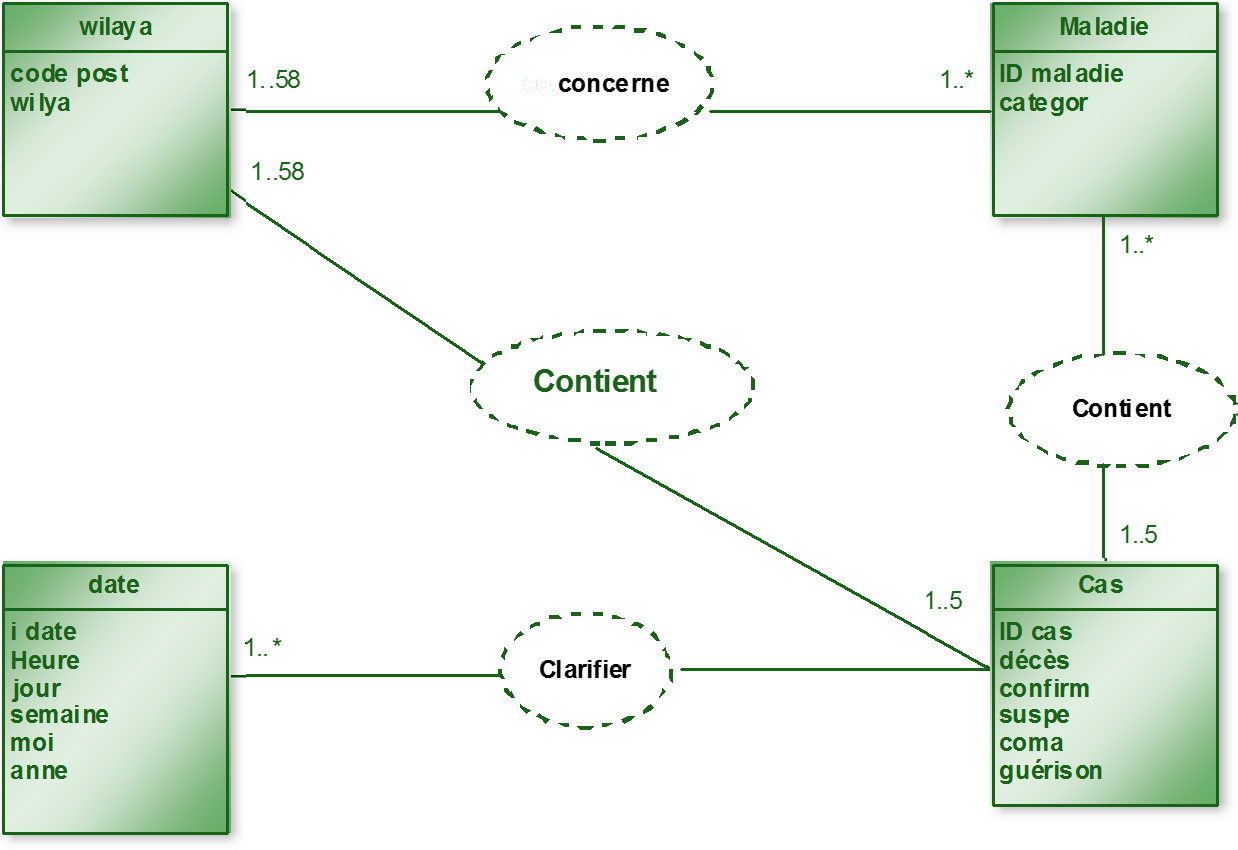
\includegraphics[width=\textwidth]{Chapitre3/entitymodel.png}}
        \caption{\label{fig:my-label} The association entity model}
     \end{figure}
     

\section{Choose a good web host}
Domain name is like the address and the CMS is like the materials you build your site with, but the web host is the actual parcel where your website exists online.\\
Some are free and come with bandwidth limitations or built-in ads, but there are also commercial options that work much better. Many hosts also provide server security features that can better protect your site data.\\
Our project is hosted in github Pages.


\section{Use a firewall}
As soon as your website is online, it is exposed to cyber threats. Automated bots search for vulnerable websites, and newly created sites are a particularly tempting target.\\

Adding a web application firewall (WAF), such as Cloudbric, Incapsula, or Cloudflare, will secure your website before attacks start.

\newpage
\section{Database schema:}
Above a schema of our Database 

\begin{figure}[!htb]
        \center{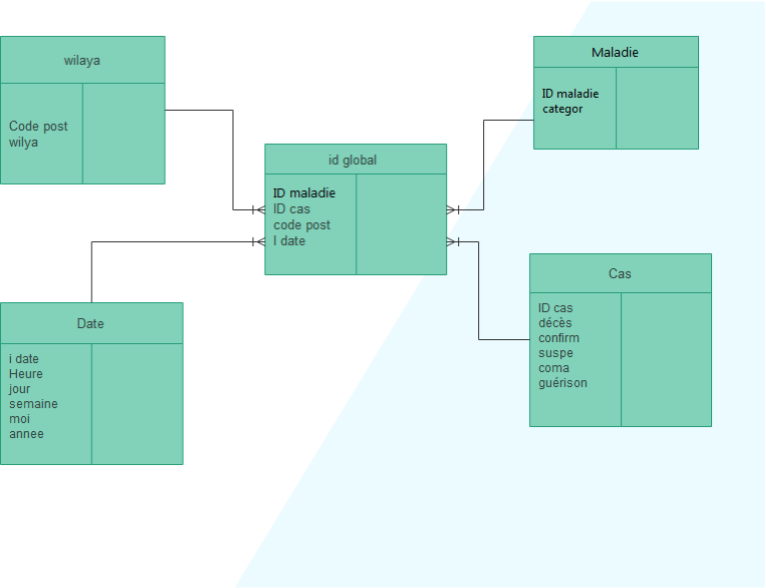
\includegraphics[width=\textwidth]{Chapitre3/db.png}}
        \caption{\label{fig:dbschema} Db Schema}
     \end{figure}
\newpage     
\section{HCI (IHM)}
According to the basic criteria of the ergonomics of the interfaces \cite{bastien1998ergonomie}, we build our Webapp as a dasshoard for a \textit{Guidance}, \textit{Explicity} with charts and Maps, \textit{Adaptability} 
\begin{figure}[!htb]
        \center{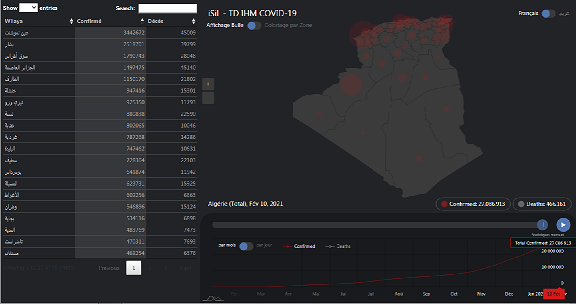
\includegraphics[width=\textwidth]{Chapitre3/dzdash.png}}
        \caption{\label{fig:dashboard} DashBoard}
     \end{figure}

\chapter*{General Conclusion}
In our project, we have presented some important theoretical and practical principles to keep in mind when designing a data visualization and preventing of Covid-19 propagation, learning common pitfalls and helpful tricks along the way. As we have seen, developing an effective and ethical data visualization is a complex process. \\

We noticed The Benefits of Data Visualization :\\
\textbf{Correlations in Relationships} Without data visualization, it is challenging to identify the correlations between the relationship of independent variables. By making sense of those independent variables, we can make better business decisions. \\

\textbf{Trends Over Time:} While this seems like an obvious use of data visualization, it is also one of the most valuable applications. It’s impossible to make predictions without having the necessary information from the past and present. Trends over time tell us where we were and where we can potentially go.\\

\textbf{Frequency:} Closely related to trends over time is frequency. By examining the rate, or how often, customers purchase and when they buy gives us a better feel for how potential new customers might act and react to different marketing and customer acquisition strategies. 
Examining the Market: Data visualization takes the information from different markets to give you insights into which audiences to focus your attention on and which ones to stay away from. We get a clearer picture of the opportunities within those markets by displaying this data on various charts and graphs.\\

\textbf{Risk and Reward: }Looking at value and risk metrics requires expertise because, without data visualization, we must interpret complicated spreadsheets and numbers. Once information is visualized, we can then pinpoint areas that may or may not require action.\\

\textbf{Reacting to the Market:} The ability to obtain information quickly and easily with data displayed clearly on a functional dashboard allows businesses to act and respond to findings swiftly and helps to avoid making mistakes.\\

For governments and researchers looking to communicate public health information, finding out how simple data visualisations influence the public is now more pressing than ever.

%\chapter*{Annexe}
\addcontentsline{toc}{chapter}{Annexe}
\bibliographystyle{plain} 
\bibliography{Bibliographie/BibliographieBDD}
\addcontentsline{toc}{chapter}{Bibliographie}

%-----------------Fin Zone 5: fin de la numérotation avec les chiffres arabs---------------------

\end {document}